\section{(Q5) - Question \#5}
\label{sec:Q5}

Write a computer code for Test Case 1 (Handout \#4, p. 352) using both Steger-Warming and van Leer flux-vector splitting methods, and compare your numerical results with the exact solutions at $t = 0.01 $ for $-10 \le x \le 10$ in terms of density, velocity, pressure, Mach number.


\subsection{Code implementation}

The code for this question is implemented in \texttt{MATLAB} and can be found in the attached files to this report.

Both the Steger-Warming and van Leer flux-vector splitting methods are implemented for the 1D Euler equations.
As for the order of the interpolation scheme used to compute the fluxes at the cell interfaces, the code allows for the selection of either a zero-order upwind scheme or a first-order linear upwind scheme.

% We leave here the function used to compute the fluxes at the cell center for both the Steger-Warming and van Leer flux-vector splitting methods.

% \lstinputlisting[
%     language=Matlab,
%     caption=Steger-Warming flux-vector splitting methods based on eigenvalues splitting.,
% ]{files/compute_flux_SW.m}

% \lstinputlisting[
%     language=Matlab,
%     caption=Van Leer flux-vector splitting methods based on Mach number splitting.,
% ]{files/compute_flux_VL.m}


\subsection{Results}

The results of the simulation are consistent with the exact solution provided with the assignment request.

In the following figures, we can see the results of the simulation for the Steger-Warming and van Leer flux-vector splitting methods for a mesh of 50 and 400 cells.

The computed solutions (black) have been interpolated using a zero-order upwind scheme (UDS).
Exact solution are represented in red.

\begin{figure}[H]
    \centering
    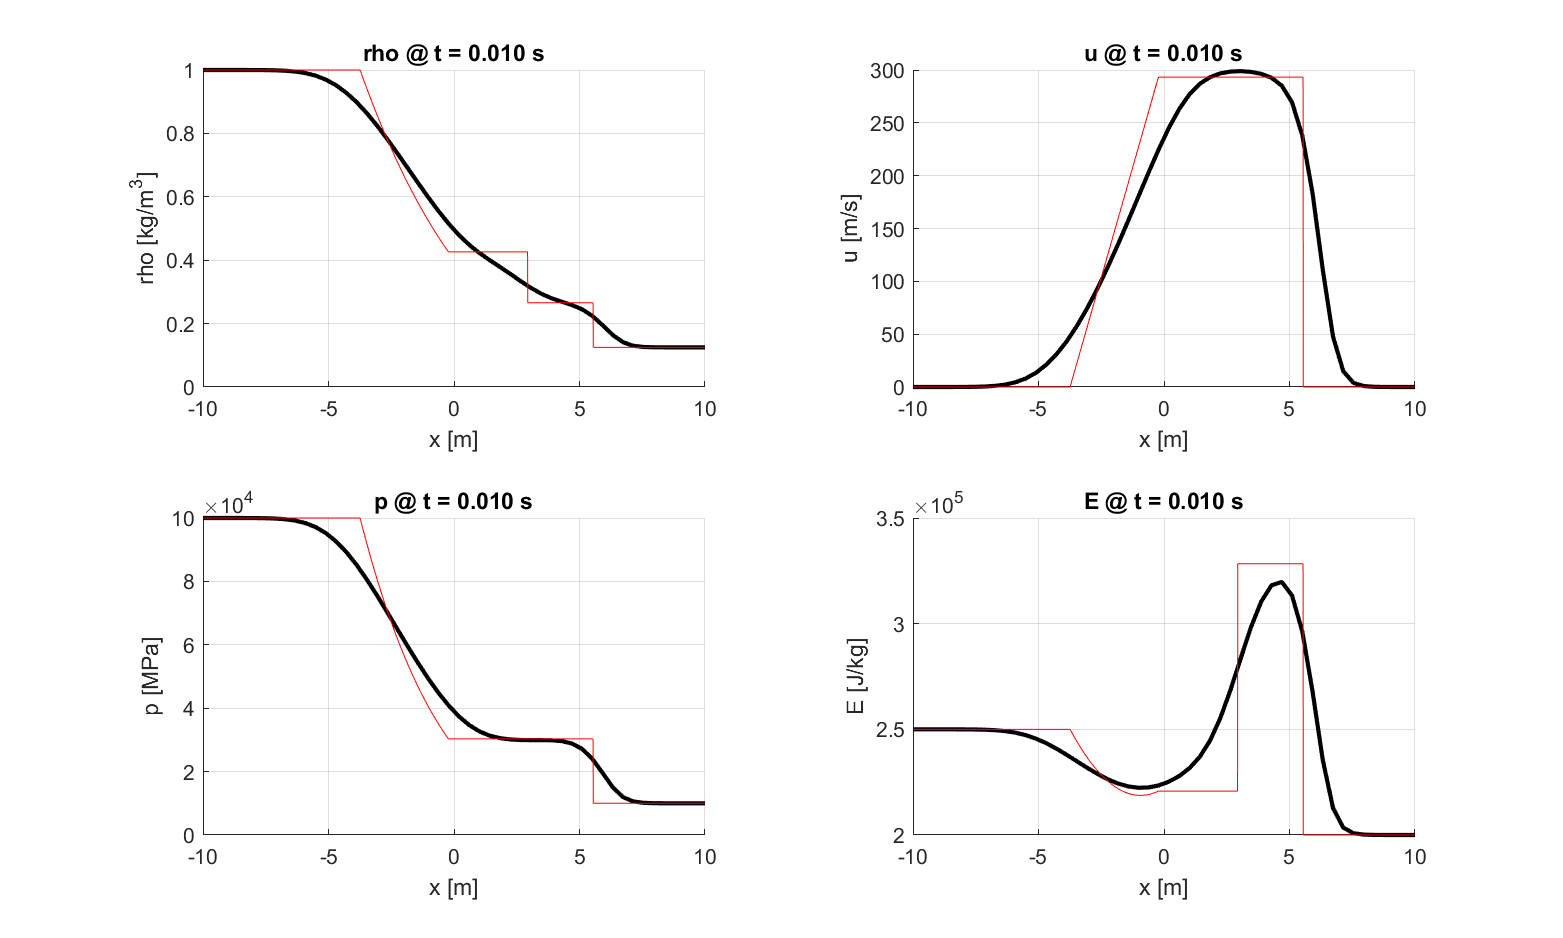
\includegraphics[width=\textwidth]{img/states/SW50.png}
    \caption{Steger-Warming flux-vector splitting method with 50 cells mesh.}
    \label{fig:SW50}
\end{figure}

\begin{figure}[H]
    \centering
    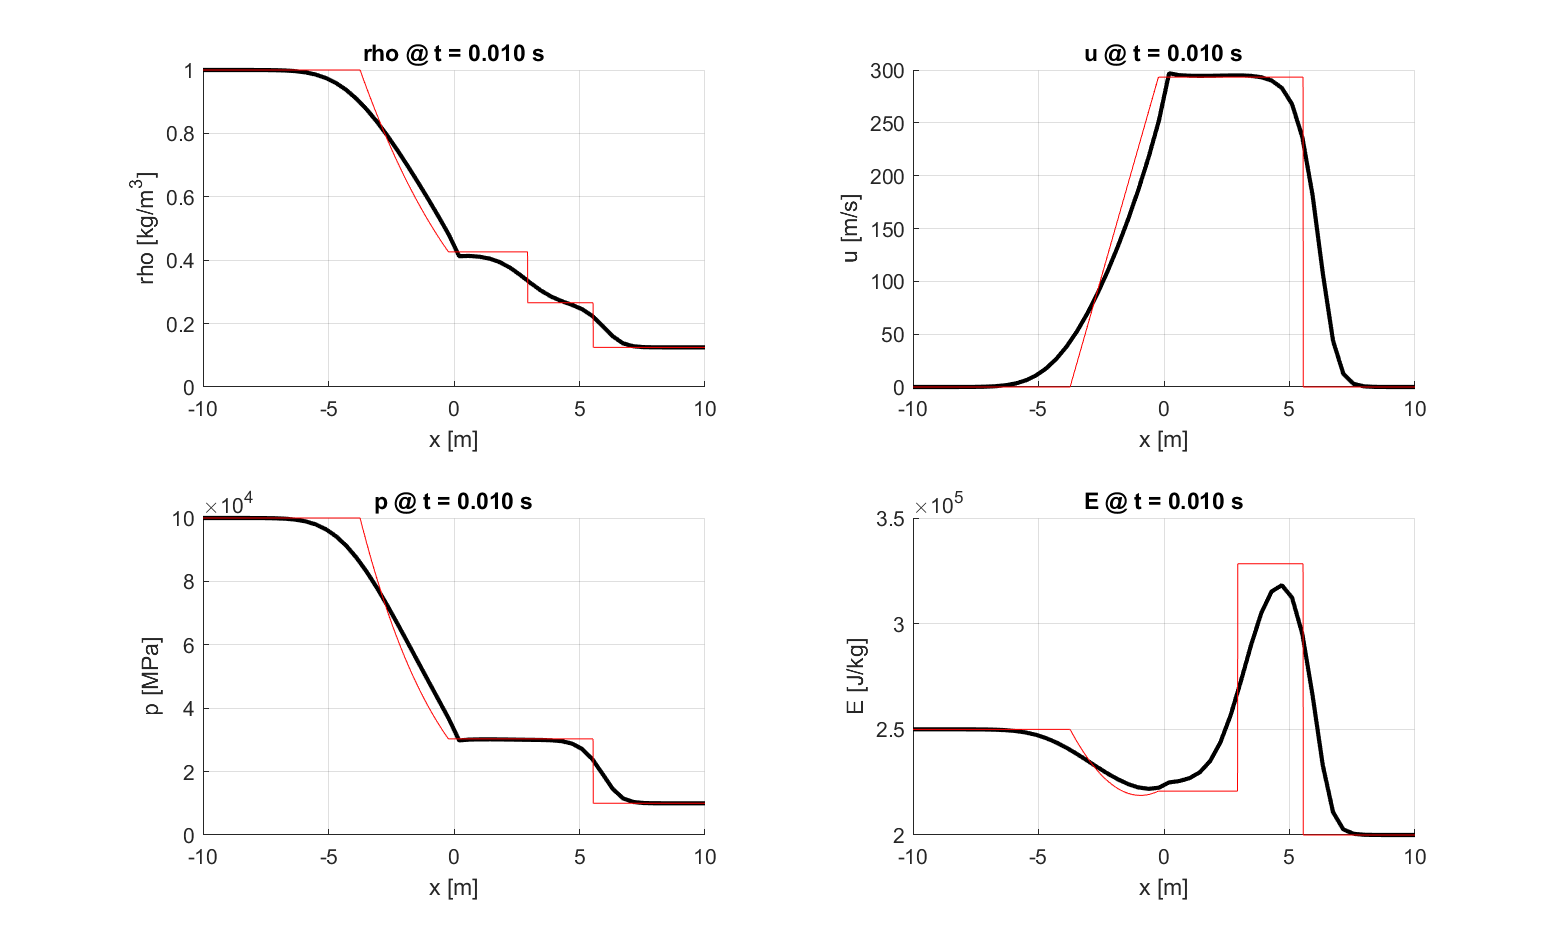
\includegraphics[width=\textwidth]{img/states/VL50.png}
    \caption{Van Leer flux-vector splitting method with 50 cells mesh.}
    \label{fig:VL50}
\end{figure}

\begin{figure}[H]
    \centering
    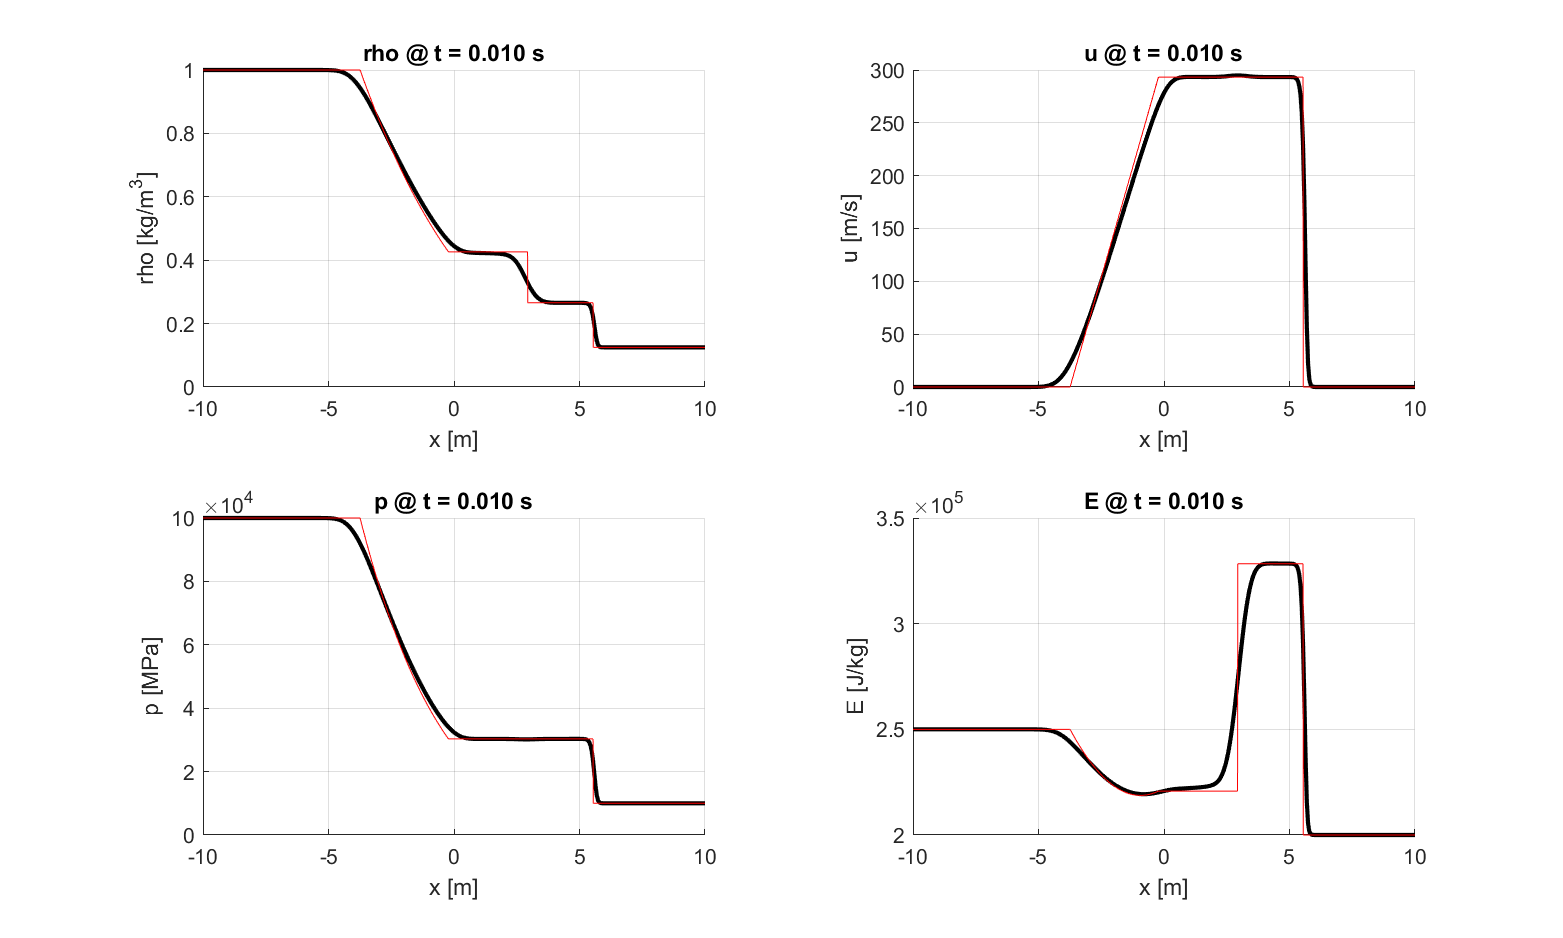
\includegraphics[width=\textwidth]{img/states/SW400.png}
    \caption{Steger-Warming flux-vector splitting method with 400 cells mesh.}
    \label{fig:SW400}
\end{figure}

\begin{figure}[H]
    \centering
    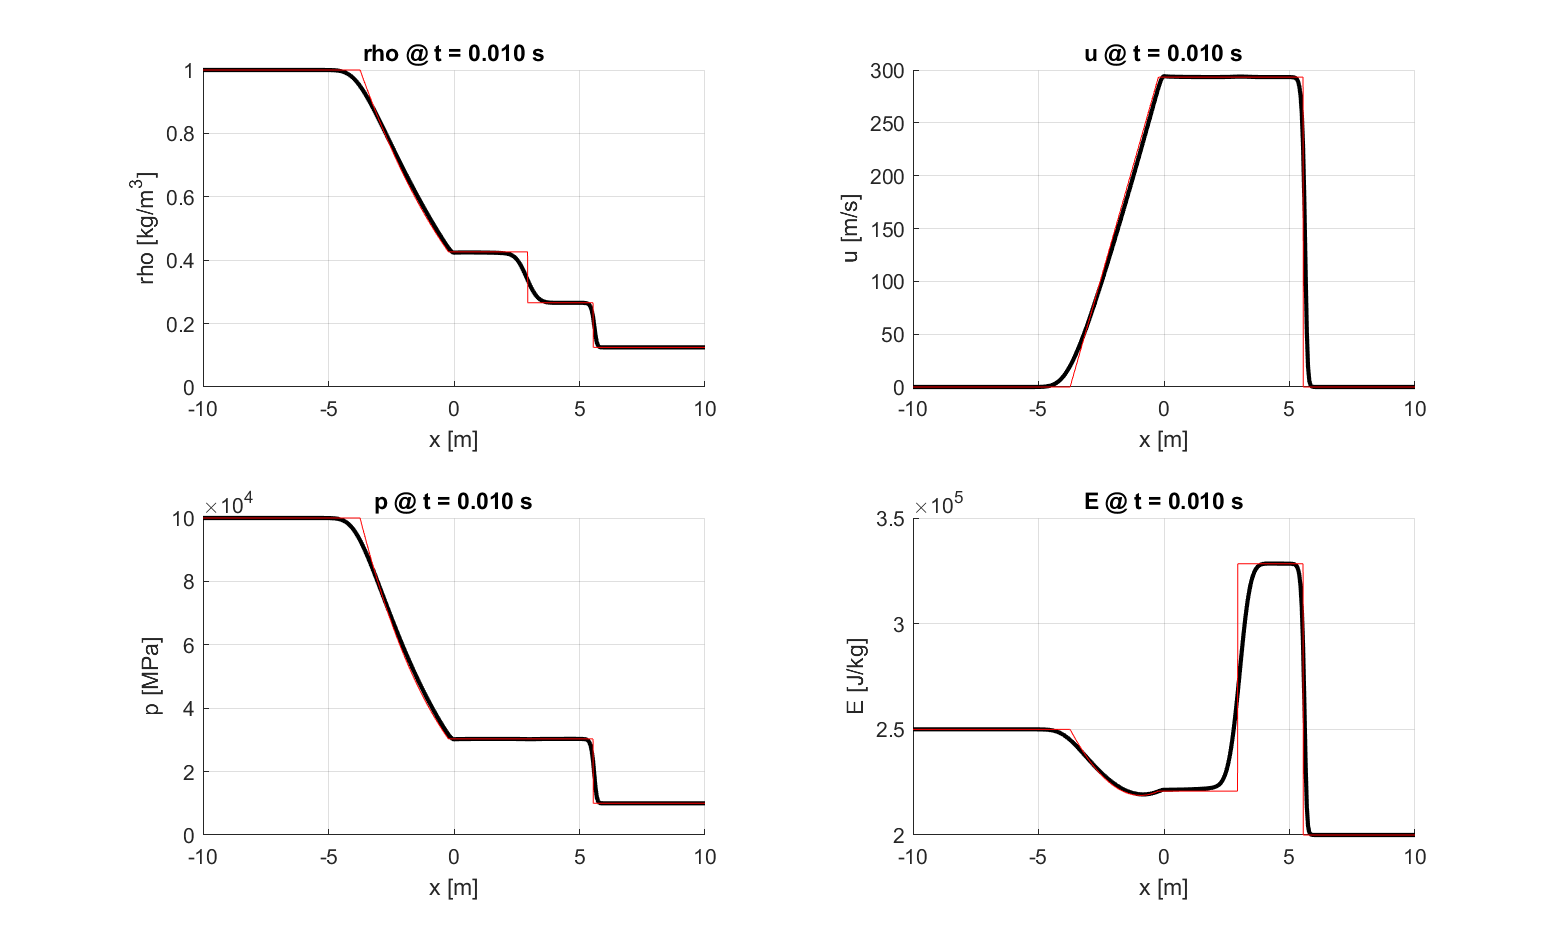
\includegraphics[width=\textwidth]{img/states/VL400.png}
    \caption{Van Leer flux-vector splitting method with 400 cells mesh.}
    \label{fig:VL400}
\end{figure}


\subsubsection{Steger-Warming vs. Van Leer splitting methods}

As we can see observing Figures \ref{fig:SW50} and \ref{fig:VL50}, the Steger-Warming method tends to be more diffusive than the van Leer method, which is more accurate in capturing the shock wave.
In particular, by observing the step ahead of the shock wave (i.e., the region behind the contact point and the expansion wave), we can see that the Steger-Warming method tends to over-diffuse the solution and doesn't capture the shock wave, while the van Leer method is more accurate in capturing the discontinuity between the two regions.

\begin{figure}[H]
    \centering
    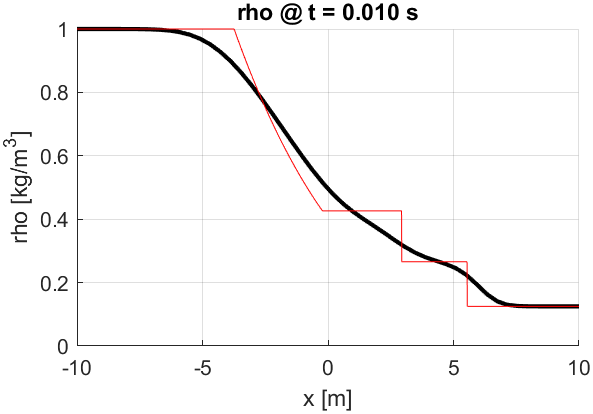
\includegraphics[width=.6\textwidth]{img/SW50_rho.png}
    \caption{Density computed with Steger-Warming flux-vector splitting method (50 cells mesh).}
    \label{fig:SW50_zoom}
\end{figure}

\begin{figure}[H]
    \centering
    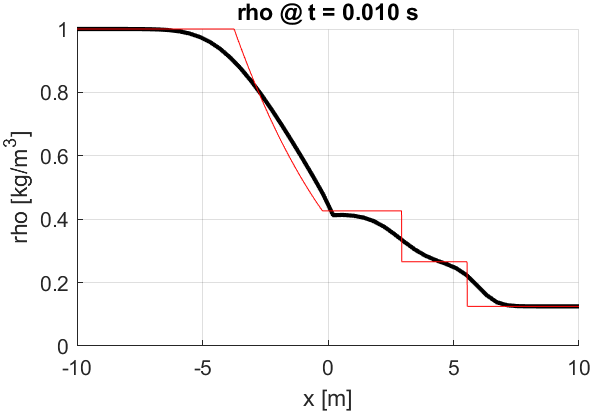
\includegraphics[width=.6\textwidth]{img/VL50_rho.png}
    \caption{Density computed with van Leer flux-vector splitting method (50 cells mesh).}
    \label{fig:VL50_zoom}
\end{figure}


\subsubsection{Order of the interpolation scheme (UDS vs. LUDS)}

The code allows for the selection of either a zero-order upwind scheme (UDS) or a first-order linear upwind scheme (LUDS) to compute the fluxes at the cell interfaces.

However, as also explained in literature, the first-order linear upwind scheme tends to be unstable, generating strong oscillations at the discontinuity regions.

In the following, we can see the results of the simulation for the Steger-Warming method and the van Leer method with a limited first-order linear upwind scheme (LUDS) for a 50 cells mesh.
In particular, the adopted interpolation scheme is the following:

\begin{equation}
    U_e = U_i + \frac{1}{4} \left( U_i - U_{i-1} \right)
\end{equation}

Notice the weight of the interpolation scheme is set to $\frac{1}{4}$ to limit the oscillations generated by the complete first-order linear upwind scheme.

\begin{figure}[H]
    \centering
    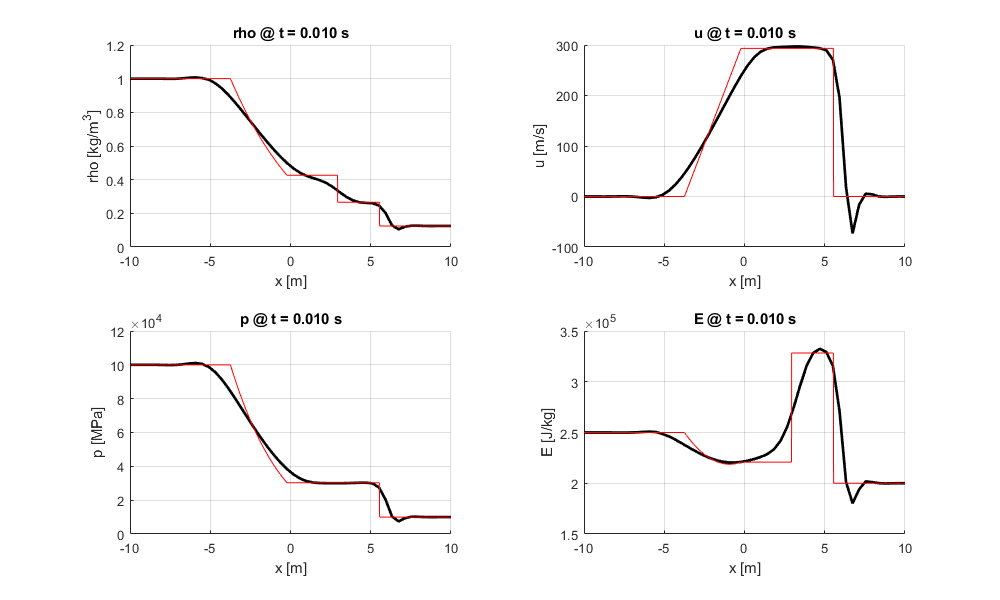
\includegraphics[width=\textwidth]{img/SW50_LUDS.png}
    \caption{Steger-Warming flux-vector splitting method with 50 cells mesh and limited LUDS interpolation scheme.}
    \label{fig:SW50_LUDS}
\end{figure}

\begin{figure}[H]
    \centering
    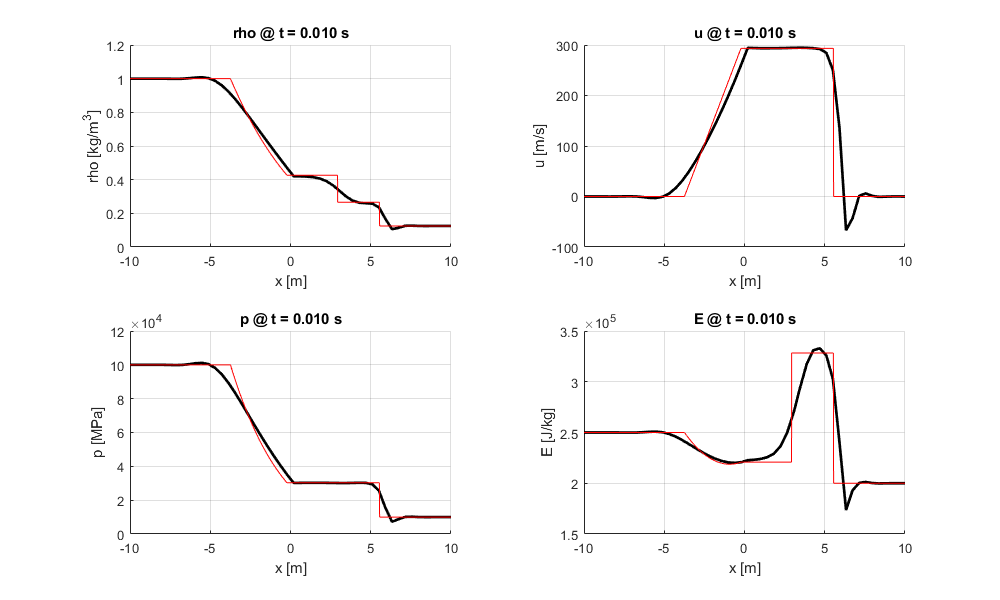
\includegraphics[width=\textwidth]{img/VL50_LUDS.png}
    \caption{Van Leer flux-vector splitting method with 50 cells mesh and limited LUDS interpolation scheme.}
    \label{fig:VL50_LUDS}
\end{figure}

In Figures \ref{fig:SW50_LUDS} and \ref{fig:VL50_LUDS}, the oscillations generated by the first-order linear upwind scheme are visible, especially in the plot of the velocity and total energy.